\subsection{Numerical experiments}\label{sec:exps}
In the previous sections we proved the convergence of \SP{} in the case where the mask is formed with a high probability $\pi$. In this section, we present numerical results providing empirical evidence on a faster execution of \SP{} with lower communication cast than if the mask is not used.




%%%%%%%%%%%%%%%%%%%%%%%%%%%%%%%%%%%%%%%%%%%%%%%%%%%%%
\subsubsection{Experimental setup}
%%%%%%%%%%%%%%%%%%%%%%%%%%%%%%%%%%%%%%%%%%%%%%%%%%%%%


In our experiments, we consider $\ell_1-\ell_2$-regularized Logistic Regression surrogate loss that is common to many machine learning and signal processing applications and which can be minimized in a distributed way. With respect to our composite learning problem \eqref{eq:pb_l1}, that is~:
\begin{equation}\label{eq:log_reg}
    \forall i\in\{1,\ldots,M\}, f_i(\w)= \frac{1}{|\mathcal{S}_i|}\sum_{(\obs_j,y_j)\in \data_i}\left[\log\left(1 + e^{-y_j\obs_j^\top \w}\right) + \frac{\lambda_2}{2}\|\w\|_2^2 \right]
\end{equation}
where $\data_i=(\obs_j,y_j)_{j\in\{1,\ldots,|\mathcal{S}_j|}\in (\RR^n\times \{-1,+1\})^{|\data_j|}$ is the sub-part of the training set stored in the worker machine $i\in\{1,\ldots,M\}$. %We fixed the hyperparameter $\lambda_2$ of the $\ell_2$ norm in \eqref{eq:log_reg} to $\lambda_2=10^{-3}$.



\begin{table}[b]
\begin{center}
\begin{tabular}{lccccc}
\hline 
Dataset              & ~~~~~~$m$~~~~~~ & ~~~~~~$n$~~~~~~ & ~~$\lambda_1$~~ & ~~$\lambda_2$~~ & $|\supp(\w^\star)|$ in (\%) \\
\hline
\vspace{1mm}{madelon}         &{$2000$} & {$500$} & $2\times10^{-2}$ & $10^{-3}$ & $7$  \\%$10^{-3}$ & $35$  \\
 %\hline%$10^{-3}$ &  $7$ \\ 
\vspace{1mm}{real-sim}    & {$72309$} & {$20958$} & $10^{-4}$ & $10^{-3}$ & $8.6$ \\%$10^{-3}$ &  $60$  \\
%\hline %$10^{-3}$ &  $0.5$  \\ 
{rcv1\_train}    & {$20242$} & {$47236$} & $10^{-4}$ & $10^{-3}$ & $4.1$ \\%$10^{-3}$ &  $29$  \\
\hline %$10^{-3}$ &  $0.25$  \\\hline
\end{tabular}
\end{center}
\caption{Statistics of datasets used in our experiments; $m$, $n$, $\lambda_1$, $\lambda_2$ and support are respectively the size of the training set, the number of parameters, the hyperparmeters corresponding to $\ell_1$ and $\ell_2$ regularization terms and the percentage of non-zero entries of the final solution; $\supp(\w^\star)$.}
\label{tab:datasets}
\end{table}

We performed experiments on three publicly available datasets\footnote{\url{https://www.csie.ntu.edu.tw/~cjlin/libsvmtools/datasets/}}. Each dataset is normalized by dividing each feature characteristic by the maximum of the absolute value in the column using the scikit-learn Transformer API.\footnote{\url{https://scikit-learn.org/stable/modules/generated/sklearn.preprocessing.normalize.html}} In Table~\ref{tab:datasets}, we present some statistics for these datasets as well as the percentage of no-zero entries of the final parameter ($\supp(\w^\star)$). 
For the communications between the master and the workers, we used the message passing interface for Python (MPI4py)\footnote{\url{https://mpi4py.readthedocs.io/en/stable/citing.html}}. We compared our approach \SP{} with its direct competitor \dave~\cite{ICML18} which is also a delay-independent asynchronous technique with constant stepsize but does not use a sparsification mask. For comparisons, we plot objective values as their relative distance to the optimum, referred to as suboptimality, with respect to time, and also with respect to iterations and the number of exchanges for different values of the probability $\pi$ used in the mask. We also present the dependence of sparsity of iterates to the number iterates. 


%%%%%%%%%%%%%%%%%%%%%%%%%%%%%%%%%%%%%%%%%%%%%%%%%%%%%%%%%%%%
\subsubsection{Speed of convergence.} 
%%%%%%%%%%%%%%%%%%%%%%%%%%%%%%%%%%%%%%%%%%%%%%%%%%%%%%%%%%%%
\begin{figure}[b!]
\begin{tabular}{cc}
\multicolumn{2}{c}{\vspace{-4pt}
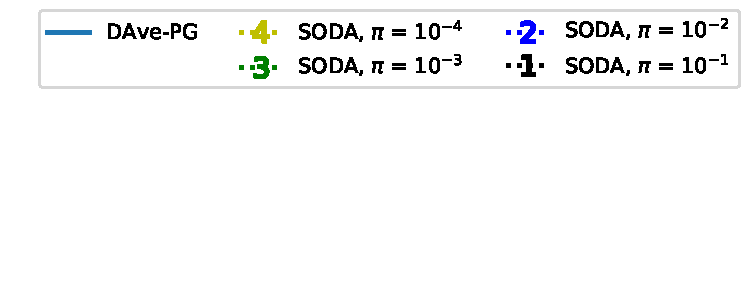
\includegraphics[width = 0.96\textwidth]{SODA/Figs/legend.pdf}}\\
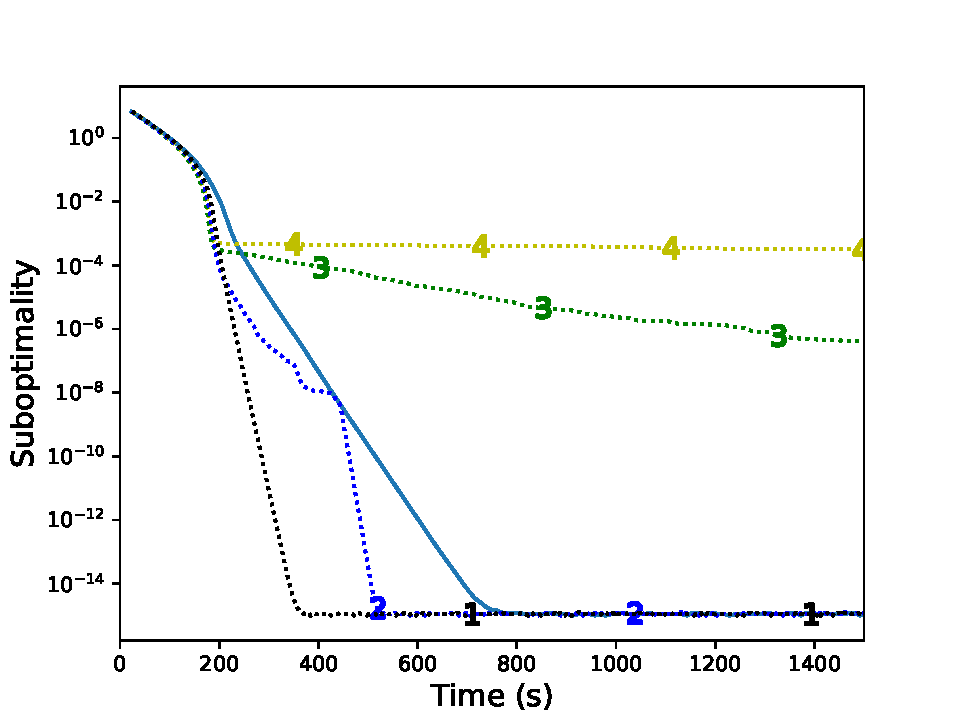
\includegraphics[width = 0.5\textwidth]{SODA/Figs/real-sim_20w_00001_0001_fun_vs_time_log.pdf} & 
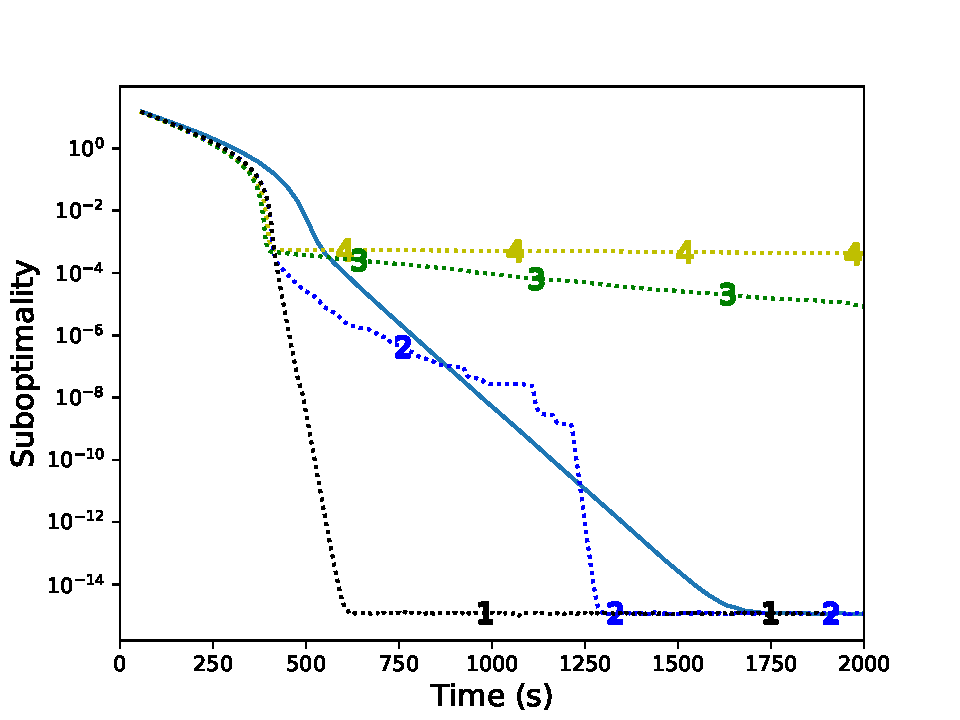
\includegraphics[width = 0.5\textwidth]{SODA/Figs/rcv_20w_00001_0001_fun_vs_time_log.pdf}\\
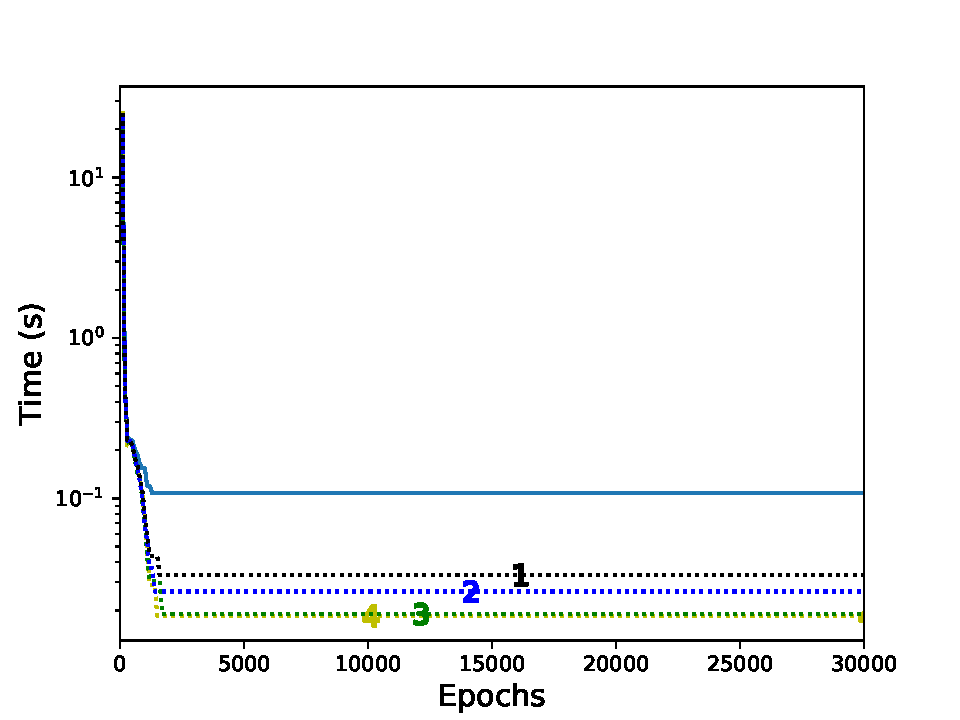
\includegraphics[width = 0.5\textwidth]{SODA/Figs/real-sim_20w_00001_0001_time_vs_ite.pdf} & 
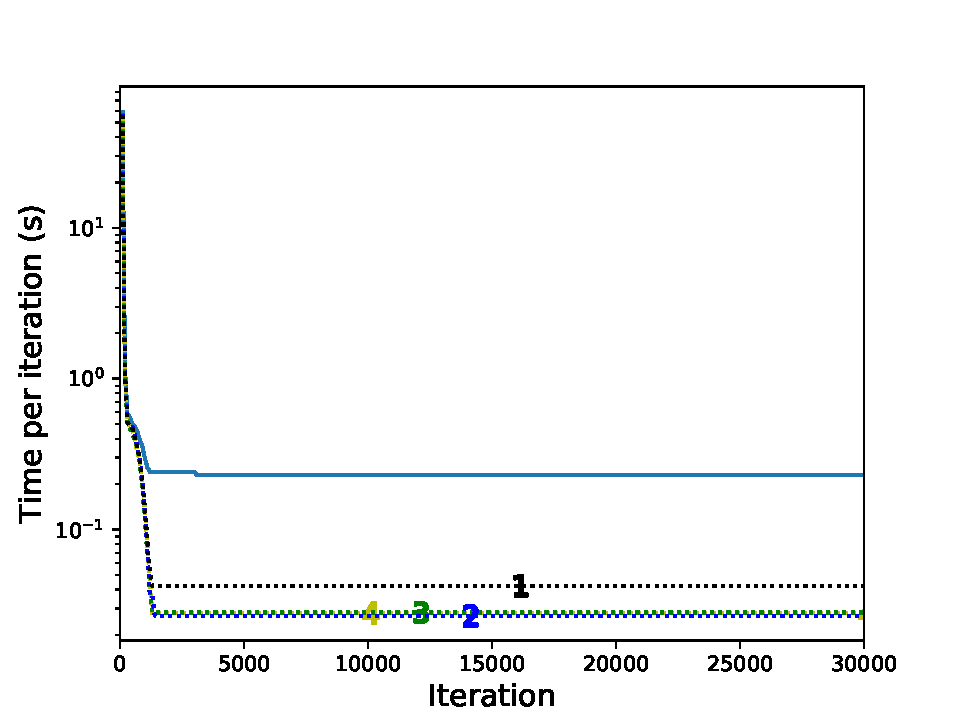
\includegraphics[width = 0.5\textwidth]{SODA/Figs/rcv_20w_00001_0001_time_vs_ite.pdf}\\
(a) real-sim & (b) rcv1\_train
\end{tabular}
    \caption{Objective loss \eqref{eq:pb_l1} suboptimality versus time in second (top) and epochs with respect to time (down), for $M=20$ workers and $\lambda_1 = 10^{-4}$ on Real\_sim and RCV1 datasets.}
    \label{fig:speed_conv}
\end{figure}
Figure \ref{fig:speed_conv} (top) presents suboptimality, as the difference between the objective function and its minimum with respect to time for the \SP{} algortihm with four values of probability $\pi$, to form the mask, and the \dave{} algorithm \cite{ICML18} with $M=20$ workers on real-sim and rcv1\_train datasets. To this end, the minimum of the loss function \eqref{eq:pb_l1}, using \eqref{eq:log_reg}, is first obtained with a precision $\epsilon=10^{-15}$. As it can be observed, for larger values of the probability $\pi$; \SP{} converges much faster than \dave{}. This is mainly because that \SP{} passes through the whole data (iteration) in lesser time than \dave{} as it can be seen in Figure \ref{fig:speed_conv} (down). For both datasets we notice that for reaching the same number of epochs, at the beginning of each plateau on the left hand side of the plots,  \SP{} put ten times less time than \dave{} for all values of the probability $\pi$.  In the supplementary, we provide more plots on all datasets for different number of workers and parameter $\lambda_1$.




%%%%%%%%%%%%%%%%%%%%%%%%%%%%%%%%%%%%%%%%%%%%%%%%%%%%%
\subsubsection{Cost of communication.}
%%%%%%%%%%%%%%%%%%%%%%%%%%%%%%%%%%%%%%%%%%%%%%%%%%%%%
We have computed the cost of communication, as the number of exchanges, between the master and the worker machines until convergence for different values of the probability $\pi$ to form the mask. In the case where $\pi$ is low, we know from the previous section that there is no guarantee that the algorithm \SP{} converges. However, note that as all workers are minimizing their local convex objectives, after one round of communication between the master and all workers, it is easy to detect when the global objective \eqref{eq:pb_l1} does not decrease at the master level and the algorithm can be stopped and restarted in this case. 
\begin{figure}[b!]
    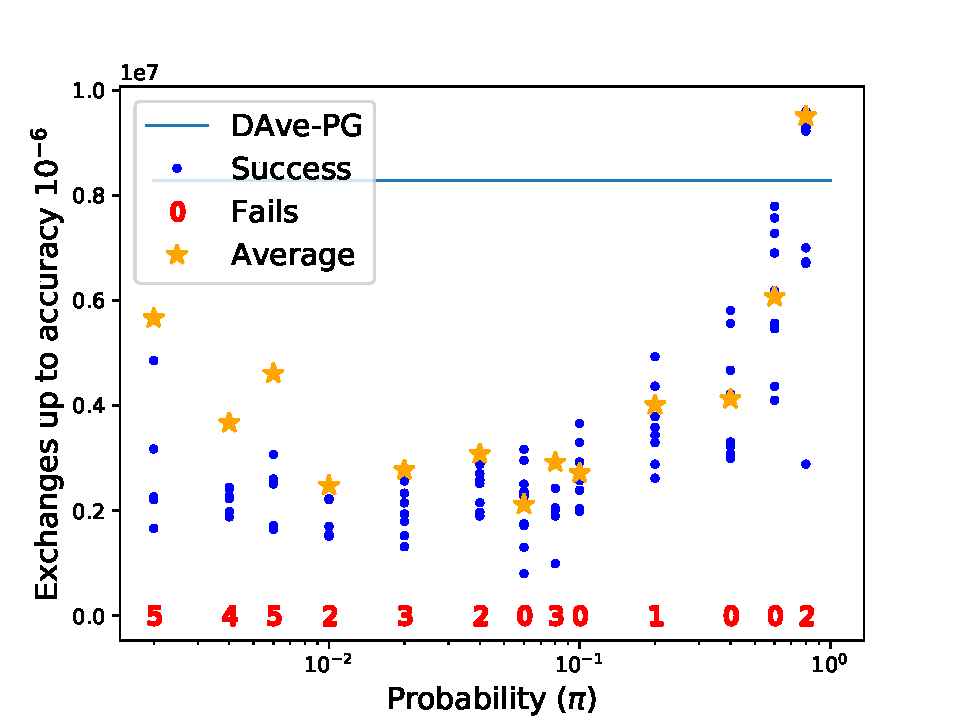
\includegraphics[width = \linewidth]{SODA/Figs/madelon_10w_002_0001_robust.pdf}
    \caption{madelon dataset, $M=10$ workers, $\lambda_1 = 0.02$.}
    \label{fig:madelon_robust}
\end{figure} 
In Figure~\ref{fig:madelon_robust} we plot the amount of exchanges between the master and the workers for different values of the probability $\pi$ used to form the mask on the madelon dataset. For each value of $\pi$; we run the algorithm $10$ times. Blue dots correspond to successful runs where the algorithm converged to the minimum of the objective \eqref{eq:pb_l1} up to the precision $10^{-15}$. Red numbers at the bottom of the figure mention the number of times when the algorithm diverged and expected amount of exchanges are shown by orange stars. In addition, we plot the line (in cyan blue) for the number of exchanges of the \dave~algorithm \cite{ICML18}. As it can be seen, in \dg{mostly} all the cases the \SP{}~algorithm converges to the minimum of \eqref{eq:pb_l1} with much less exchanges between the master and the workers than in the \dave{} algorithm. For lower values of $\pi$, the number of times where the algorithm converges is low and for larger values of $\pi$; the expected number of exchanges tends to the one of the \dave~algorithm. This figure suggests that for this dataset the best compromise between the number of convergence and number of exchanges is reached for the values of $\pi\in[0.01,0.6]$. 
\begin{figure}[t!]
\begin{tabular}{cc}
\multicolumn{2}{c}{\vspace{-4pt}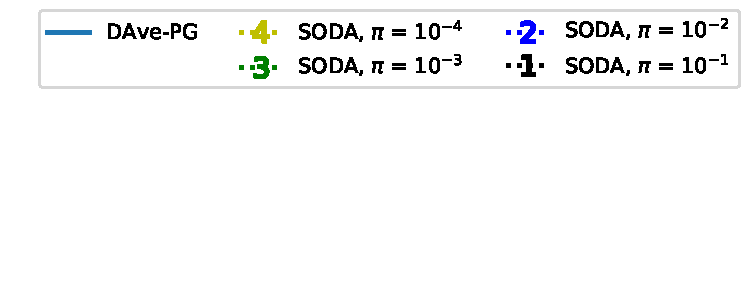
\includegraphics[width = 0.96\textwidth]{SODA/Figs/legend.pdf}}\\
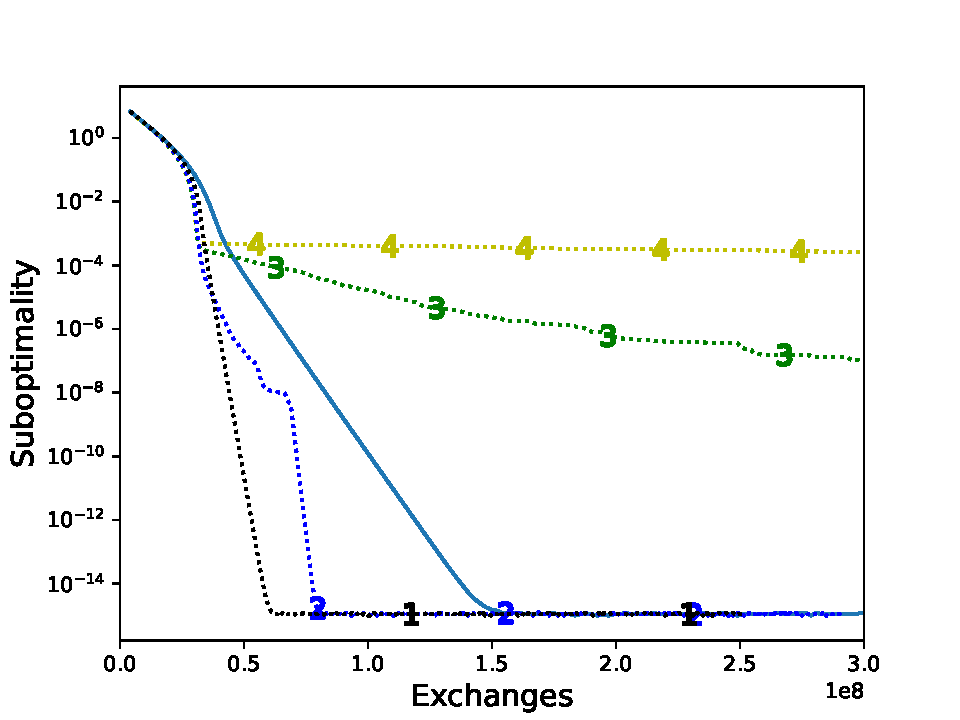
\includegraphics[width = 0.5\textwidth]{SODA/Figs/real-sim_20w_00001_0001_fun_vs_ex_log.pdf} & 
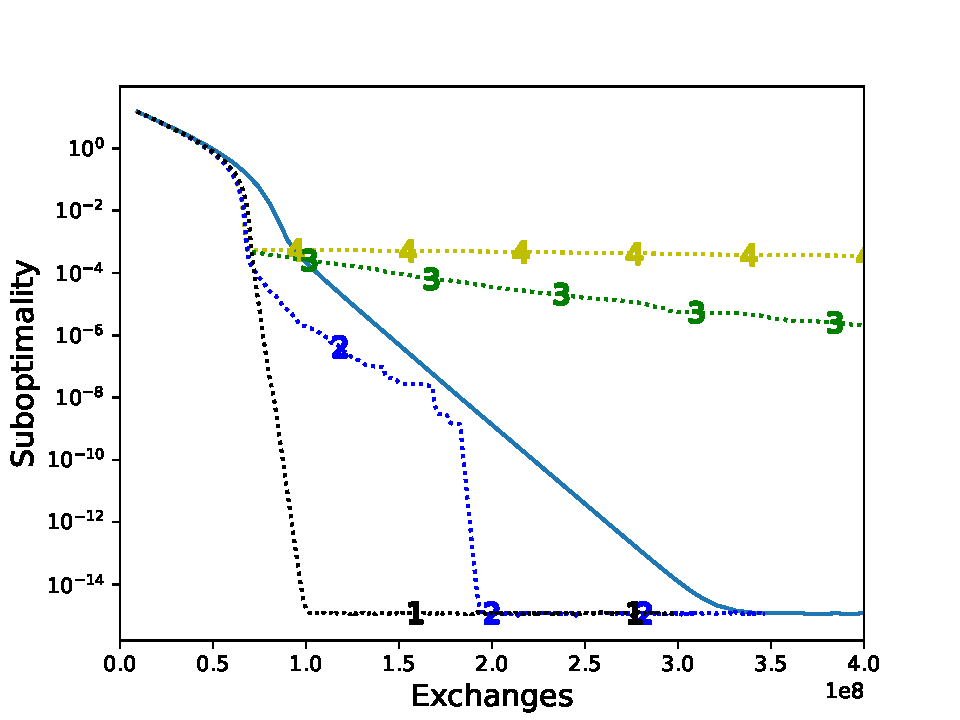
\includegraphics[width = 0.5\textwidth]{SODA/Figs/rcv_20w_00001_0001_fun_vs_ex_log.pdf}\\
(a) real-sim & (b) rcv1\_train
\end{tabular}
    \caption{Objective loss \eqref{eq:pb_l1} suboptimality versus number of exchanges, for $M=20$ workers and $\lambda_1 = 10^{-4}$ on real-sim  and rcv1\_train datasets.}
    \label{fig:communication}
\end{figure}
\begin{figure}[h]
\begin{tabular}{cc}
\multicolumn{2}{c}{\vspace{-4pt}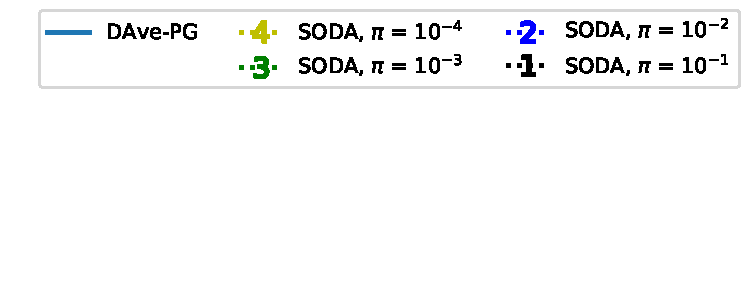
\includegraphics[width = 0.96\textwidth]{SODA/Figs/legend.pdf}}\\
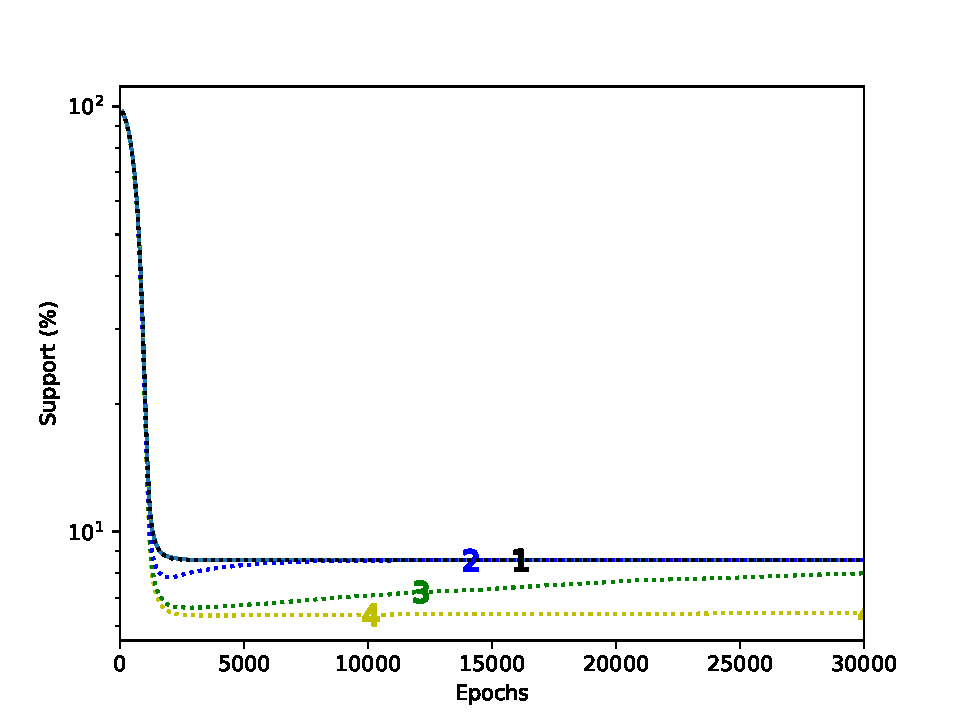
\includegraphics[width = 0.5\linewidth]{SODA/Figs/real-sim_20w_00001_0001_density.pdf} & %\label{fig:real_f_vs_e}}
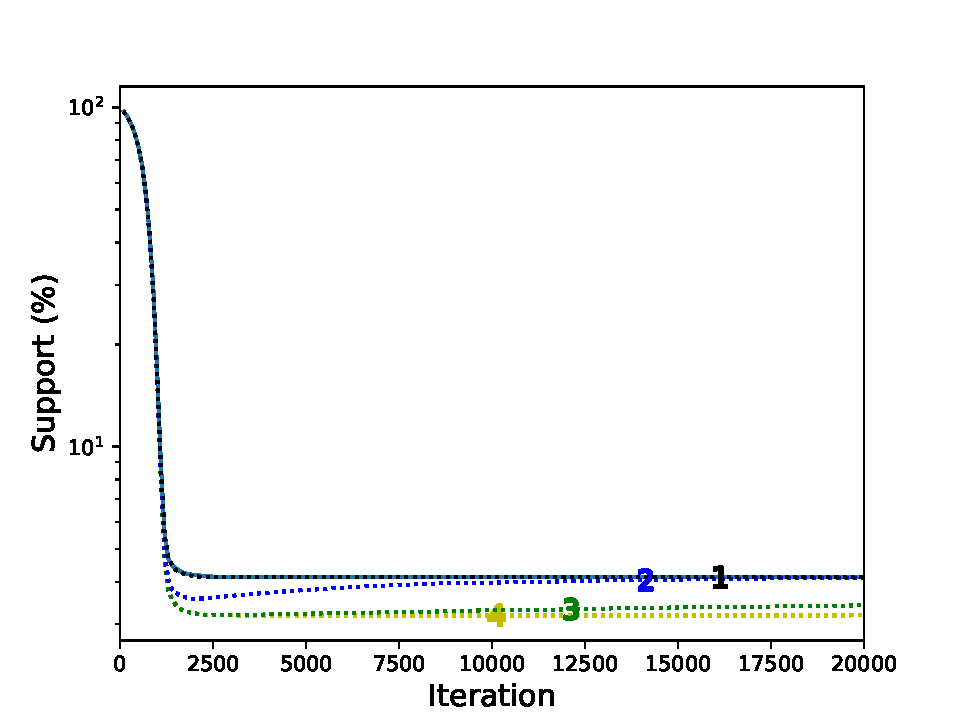
\includegraphics[width = 0.5\linewidth]{SODA/Figs/rcv_20w_00001_0001_density.pdf}\\%\label{fig:real_f_vs_t}}
(a) real-sim & (b) rcv1\_train
\end{tabular}
\caption{Evolution of sparsity versus iterations on real-sim and rcv1\_train collections with, $M=20$ workers and $\lambda_1= 10^{-4}.$}
    \label{fig:real_diff_sp}
\end{figure}
\begin{figure}[b!]
\begin{tabular}{cc}
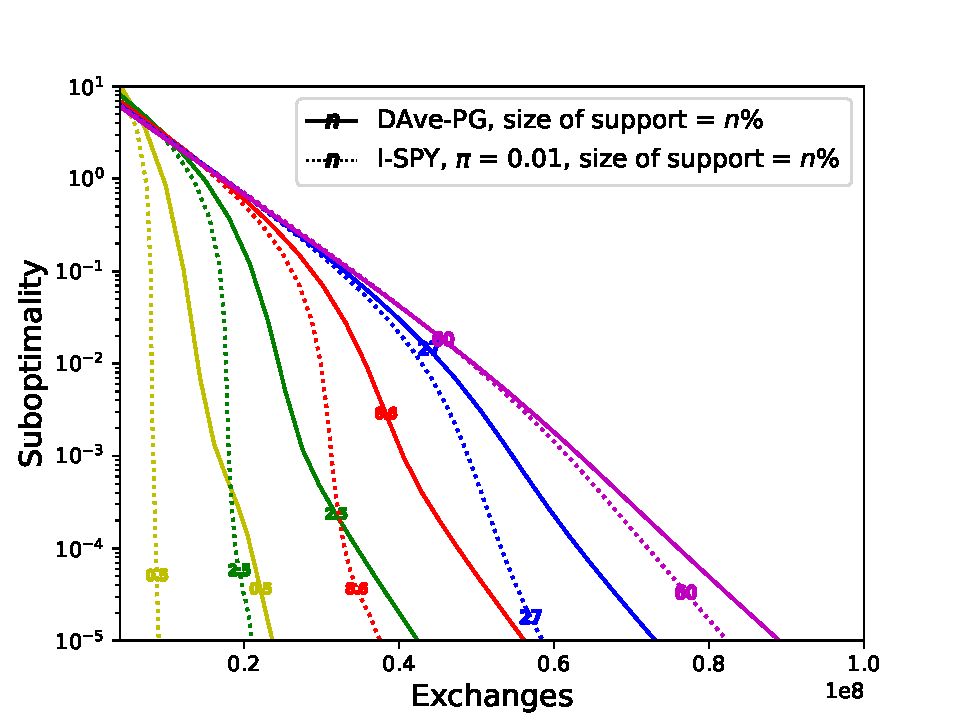
\includegraphics[width = 0.49\linewidth]{SODA/Figs/real-sim_20w_diff_sp_fun_vs_ex_log.pdf}&
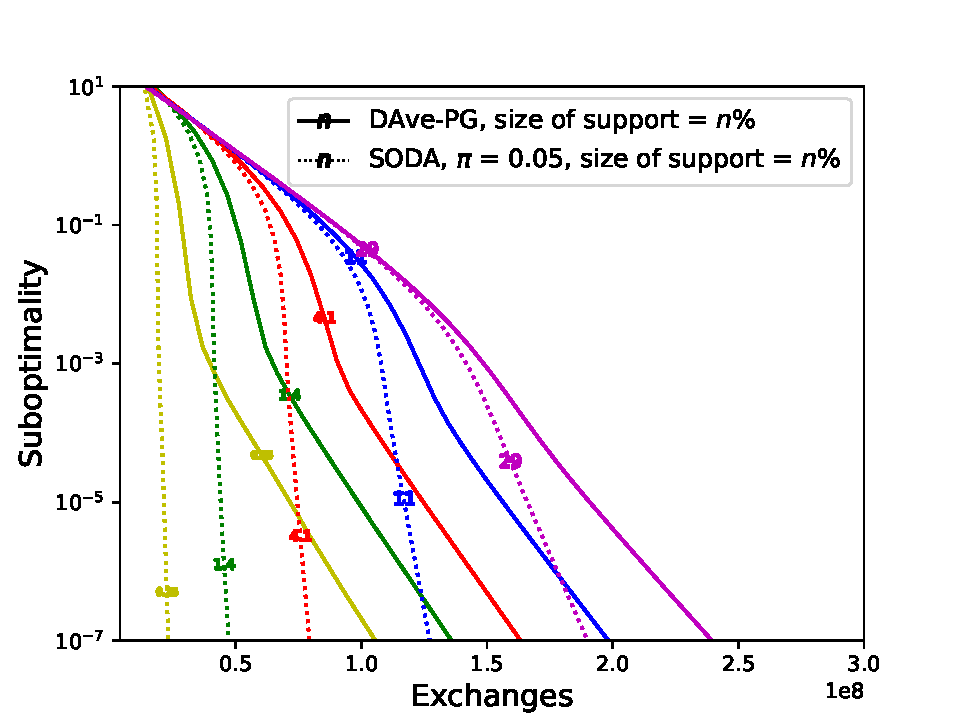
\includegraphics[width = 0.49\linewidth]{SODA/Figs/rcv1_train_20w_diff_sp_fun_vs_ex_log.pdf}\\%\label{fig:real_f_vs_t}}
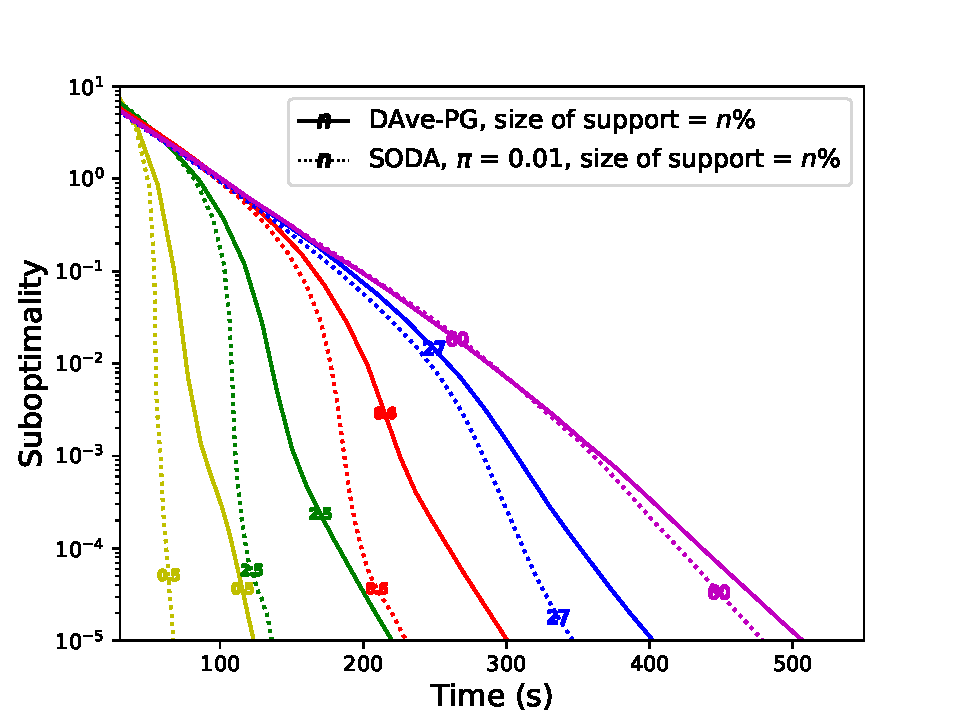
\includegraphics[width = 0.49\linewidth]{SODA/Figs/real-sim_20w_diff_sp_fun_vs_time_log.pdf}&
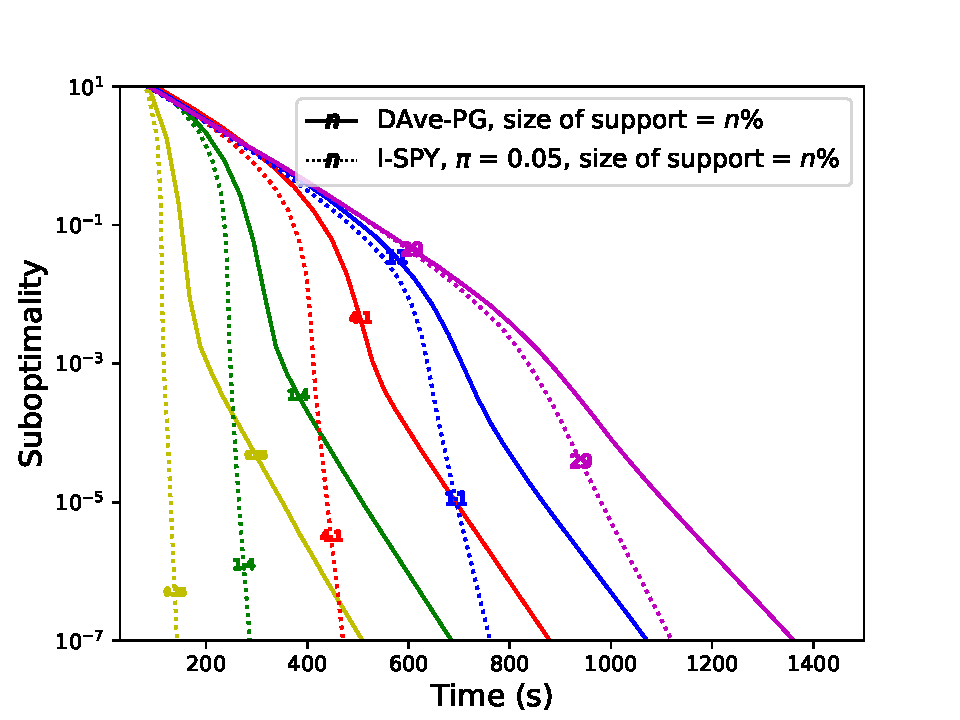
\includegraphics[width = 0.49\linewidth]{SODA/Figs/rcv1_train_20w_diff_sp_fun_vs_time_log.pdf}\\%\label{fig:real_f_vs_t}}
(a) real-sim & (b) rcv1\_train
\end{tabular}
\caption{Dependence of gain on the sparsity of the final solution}
\label{fig:different_final_sparsity}
\end{figure}
In Figure \ref{fig:communication}, we present the number of exchanges with respect to suboptimality for the \dave{} algorithm \cite{ICML18} and \SP{} with different values of the probability $\pi$ to form the mask on real-sim and rcv1\_train datasets. As it can be observed; for larger values of $\pi$, \SP{} converges faster  with much less exchanges. These plots with the ones of Figure \ref{fig:speed_conv}, suggest that if the mask is formed with a large enough probability $\pi$, the proposed algorithm converges faster with fewer exchanges and epochs to the optimum of the global objective function than without sparsification.


%%%%%%%%%%%%%%%%%%%%%%%%%%%%%%%%%%%%%%%%%%%%%%%%%%%%%
\subsubsection{Evolution of sparsity.}
%%%%%%%%%%%%%%%%%%%%%%%%%%%%%%%%%%%%%%%%%%%%%%%%%%%%%

Let us finally discuss the importance of sparsity, as the number of no-zero entries, of the final solution. Figure \ref{fig:real_diff_sp}, shows the evolution of the percentage of no-zero entries of the parameter with respect to epochs on \dg{real-sim} and \dg{rcv1\_train} datasets for $M=20$ workers and $\lambda_1=10^{-5}$. The sparsity of the solution increases over epochs for both \dave{} and \SP{} algorithms. This is mainly due to the use of the $\ell_1$ in both algorithms. This sparsification is accentuated for \SP{} by the use of the mask. From previous plots, we observed that for higher values of the probability $\pi$, the proposed algorithm converges faster to the minimum of the composite objective. From Figure \ref{fig:real_diff_sp}, it comes out that in this case, the \SP{} algorithm is able to identify the same set of informative non-zero entries, than \dave{}, at convergence for higher values of the probability $\pi$.

In Figure \ref{fig:different_final_sparsity}, we present the evolution of the functional suboptimality for two different datasets: rcv1\_train and real-sim. For both datasets we see that the gain is bigger if the final sparsity is smaller. It corresponds to the theoretical rate of Theorem \ref{th:rate_after}.

\section{Conclusion}\label{sec:conclusion}
In this chapter, we proposed an asynchronous distributed learning algorithm with sparsification. The sparsification is induced through a mask that selects a subpart of the model parameters constituted with all non-zero entries and some others chosen randomly with a fixed probability $\pi$. We analyzed the convergence property of the algorithm by showing that when $\pi$ is moderately high, the algorithm is ensured to converge for strongly convex composite objectives. In the case of small values of $\pi$, we have empirically shown on three benchmarks that when the algorithm converges, it reaches faster the minimum with much fewer communications between the master and the worker machines than if the mask is not used. This algorithm has no guarantee, and we propose its modification with theoretical proofs of convergence in the next chapter.